
\section{Dataset}
The datasets consists of 3 different edgefiles, which represents different interactions of twitterusers. Since these are are one way interactions, the datasets each represents a directed graph.\\
 In order to recreate the informationflow, the graphs must be reversed and and summed up to represent one value per edge of an interaction. In the next step those new weights had to be normalized
\section{Implementation and Result Analysis}
In this chapter we will discuss the implementation of the ICM and greedy algorithm.
\subsection{Independent Cascade Model (ICM)}
The Independent cascade model is a stochastic information diffusion model where the information go through the network in a cascade. In such a model nodes can be either active or inactive. If a node is active it means that the node is already influenced by the information in the diffusion. On the other case, the node doesn't know anything about the information and is not influenced.
The information diffusion starts as follows: At the beginning some nodes receives the information. These nodes are known as seed nodes. This nodes are automatically active. In each step an active node can influence his inactive neighbor. If no activation happens then this node will never have again a chance to influence this exact neighbor. When a neighbor is activated depends on the probability on the edge between those 2 nodes, if the edgeweight is higher than the probability, then this neighbor will be activated, and can in the next step can activate his neighbor.
\subsection{Maximizing the spread of cascades - Greedy algorithm}

With a greedy algorithm our main focus was on optimising the cycle speed to facilitate the treatment of our dataset and not having to wait half an our to get only a few seeds.
One of the first hurdle was to make the algorithm deterministic instead of stochastic for consistency. For that we're using the \href{https://docs.python.org/3.8/library/random.html#random.seed}{random.seed} from python random library, which will give us consistent generated values.

\begin{figure}[H]
    \centering
    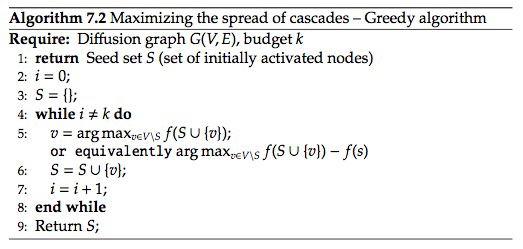
\includegraphics{Report/images/greedy_pseudo.png}
    \caption{Pseudocode of Greedy algorithm}
    \label{fig:my_label}
\end{figure}

The first implementation was relatively inefficient. The cascades were calculated from scratch for each nodes each time we were trying to determine the highest spreading node (line 5 of the pseudocode in \ref{fig:my_label}.)
To solve that we moved to calculate the activation for each nodes preemptively with \texttt{neighbors\_activation(G)} which check the potential for each node to activate its neighbours.
This accelerated the process, but was still slow. 

To optimise more, cascades were eventually move to be pregenerated to with \texttt{icm\_all(G, act)}. This gives us a dictionary of cascade for each nodes. With this the algorithm speed improve drastically. It went on my machine from 15 seconds to calculate the 3rd most activating users in our network to 12 seconds to calculate the 300th most activating user. 
\begin{figure}
\lstinputlisting[language=Python, firstline= 7, lastline=32,breaklines=true]{../greedy.py}
\end{figure}

\subsubsection{Results}

\section{Evaluation}

\subsection{ICM - Activation over time}
\subsubsection{Lower the probability}
Because of the low weights, an activation is not likely to happen. To be able to activate more nodes, we generate now a value between 0 and 0.1 and gibe them as a new probability

\subsection{Greedy algorithm - variation of budget \textit{k}}
\subsection{Pearson correlation}
To calculate the pearson coefficient we took each dataset individually and also the normalized graph.
To calculate the values we used the networkx library \textit{degree\_pearson\_correlation\_coefficient}, which gave us the following values:
\begin{center}
 \begin{tabular}{||c | c ||} 
 \hline
 Mention & -0.020746744677204432 \\
 \hline
 Reply & -0.04064928293680786\\ 
 \hline
 Retweet & 0.003181572224277474\\ 
 \hline
 Normalized & -0.020746744677204432 \\ 
 \hline
\end{tabular}
\end{center}
\subsubsection{Analysis of results}
All four values are around 0. A value of zero gives us no correlation between the nodes.  %still not complete
\subsection{Linear Threshold Model (LTM) over time}
The LTM is such a model where the weights of the edges between the nodes represent how much the nodes can affect each other
For this part of the analyse we took 30 initial active nodes.
\begin{figure}[H]
\minipage{0.4\textwidth}
    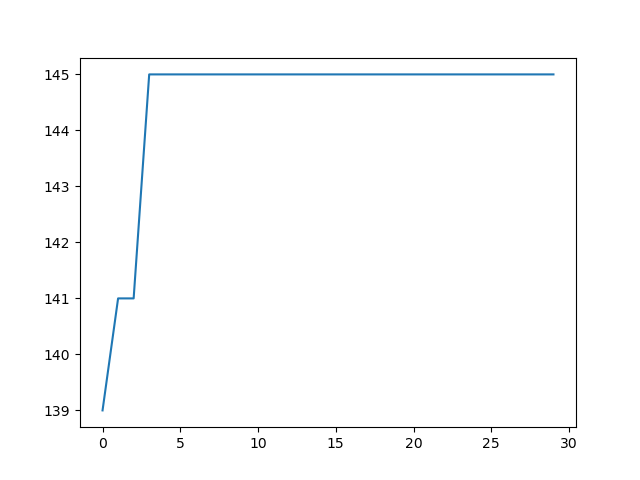
\includegraphics[width=\linewidth]{Report/images/sumLTM-0to1.png}
    \caption{Probabilities from 0 to 1}\label{fig:awesome_image1}
\endminipage\hfill
\minipage{0.4\textwidth}
    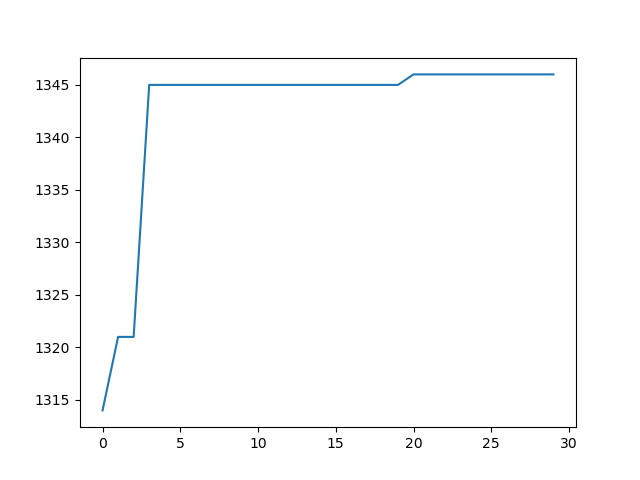
\includegraphics[width=\linewidth]{Report/images/sumLTM.png}
    \caption{Probabilities from 0 to 0.1}\label{fig:awesome_image2}
\endminipage
\end{figure}
\subsection{Discussion}

